\documentclass[11pt]{article}
\usepackage[margin=1cm]{geometry}
\usepackage{amsmath,amssymb}
\usepackage{xcolor}
\usepackage{tikz}
\usetikzlibrary{arrows.meta, shadows, decorations.pathreplacing}

\definecolor{grayTop}{RGB}{210,210,210}
\definecolor{grayBot}{RGB}{100,100,100}
\definecolor{greenTop}{RGB}{175,195,115}
\definecolor{greenBot}{RGB}{65,85,40}
\definecolor{goldTop}{RGB}{228,195,115}
\definecolor{goldBot}{RGB}{150,150,150}
\definecolor{redTop}{RGB}{235,175,160}
\definecolor{redBot}{RGB}{190,75,65}
\definecolor{accentRed}{RGB}{210,20,20}
\definecolor{accentBlue}{RGB}{15,55,200}
\definecolor{shadowGray}{RGB}{50,50,50}

\tikzset{
  databox/.style={rectangle, rounded corners=10pt, draw=black!50, thick,
    drop shadow={shadow xshift=1.5pt, shadow yshift=-2pt, opacity=0.35, fill=shadowGray},
    align=center, font=\sffamily\large, text=black!85},
  whitebox/.style={rectangle, draw=black, thick, align=center,
    font=\sffamily\normalsize},
  tagbox/.style={rectangle, draw=black, very thick, fill=white,
    font=\sffamily\bfseries, text=accentRed}
}

\begin{document}
\begin{figure}[htbp]
\centering
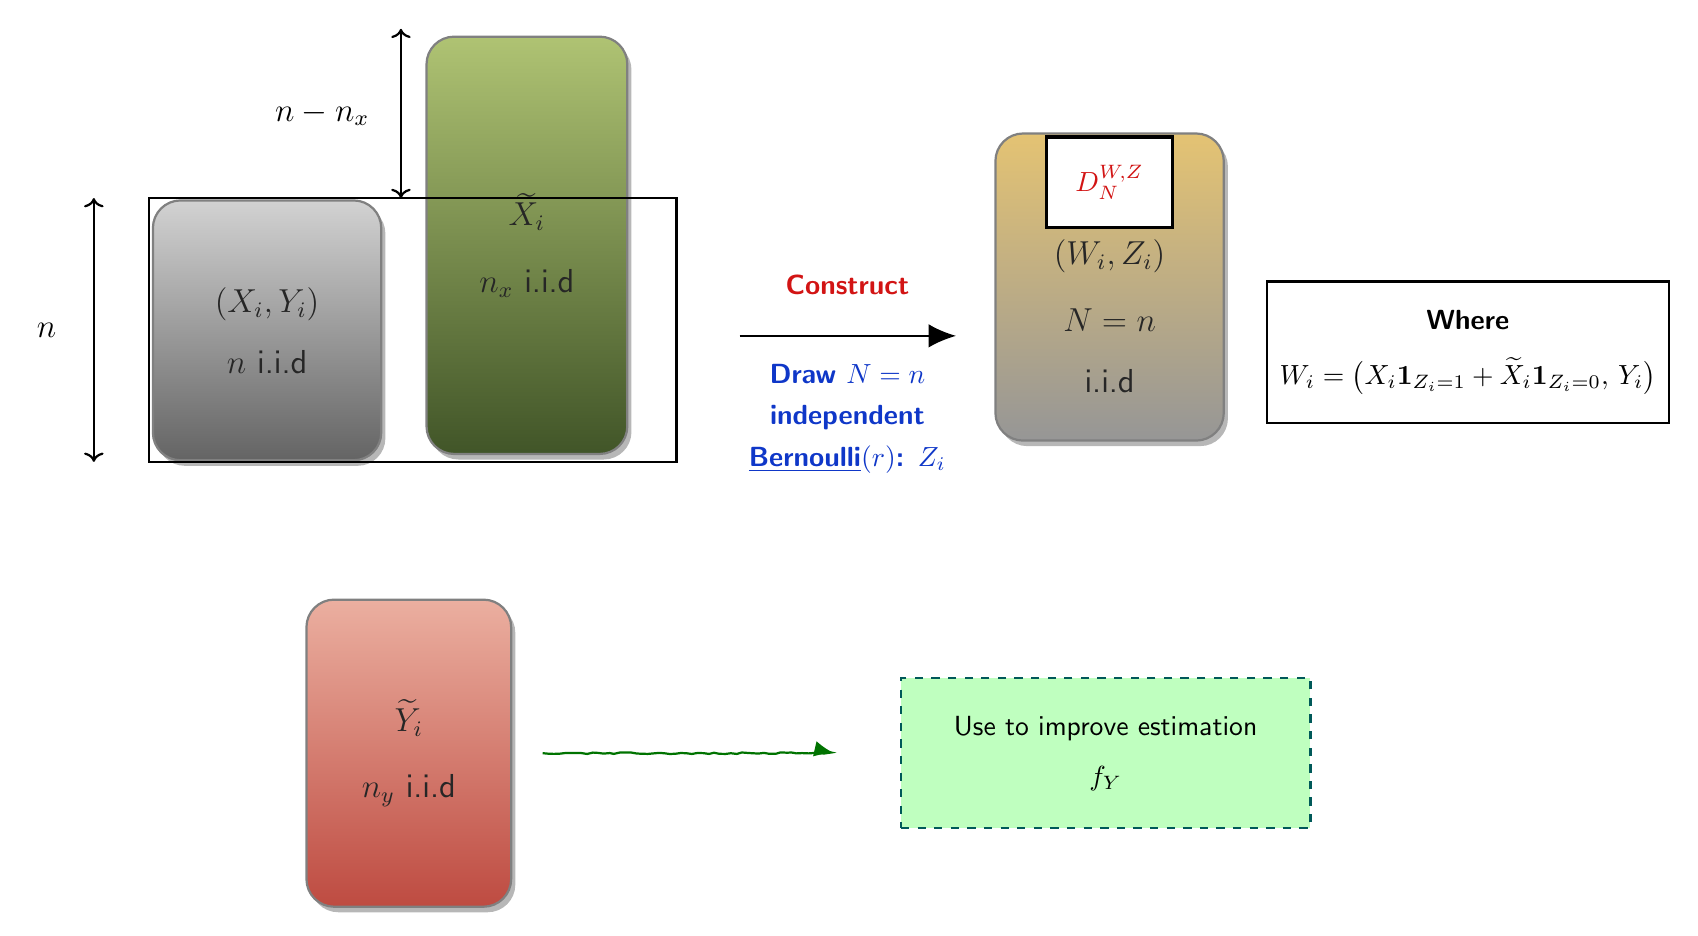
\begin{tikzpicture}[x=1cm,y=1cm]

% ================= BLOC SOURCE (haut gauche) =================
\node[databox, top color=grayTop, bottom color=grayBot,
      minimum width=2.9cm, minimum height=3.3cm] (XY) at (2.35,6.97)
  {$(X_i,Y_i)$\\[8pt] $n$ i.i.d};

\node[databox, top color=greenTop, bottom color=greenBot,
      minimum width=2.55cm, minimum height=5.3cm] (Xt) at (5.65,8.05)
  {$\widetilde{X}_i$\\[10pt] $n_x$ i.i.d};

% Cadre noir englobant (n)
\draw[black, thick] (0.85,5.30) rectangle (7.55,8.65);

% Cotation "n"
\draw[<->, thick] (0.15,5.30) -- (0.15,8.65);
\node[font=\sffamily\large] at (-0.45,6.97) {$n$};

% Cotation "n - n_x" (bien espacee au-dessus)
\draw[<->, thick] (4.05,8.65) -- (4.05,10.80);
\node[font=\sffamily\large] at (3.05,9.72) {$n-n_x$};

% ================= FLECHE CONSTRUCT =================
\draw[-{Latex[length=3.5mm,width=3mm]}, thick] (8.35,6.90) -- (11.10,6.90);
\node[font=\sffamily\bfseries, text=accentRed] at (9.72,7.55) {Construct};
\node[font=\sffamily\bfseries, text=accentBlue, align=center] at (9.72,5.85)
  {Draw $N=n$\\[3pt] independent\\[3pt] \underline{Bernoulli}$(r)$: $Z_i$};

% ================= BOITE D_N^{W,Z} =================
\node[databox, top color=goldTop, bottom color=goldBot,
      minimum width=2.9cm, minimum height=3.9cm] (DWZ) at (13.05,7.52)
  {\\[16pt] $(W_i,Z_i)$\\[10pt] $N=n$\\[8pt] i.i.d};

\node[tagbox, minimum width=1.6cm, minimum height=1.15cm] (tag) at (13.05,8.85)
  {$\mathscr{D}_N^{W,Z}$};

% ================= BOITE WHERE =================
\node[whitebox, minimum width=5.1cm, minimum height=1.8cm] (where1) at (17.6,6.69)
  {\textbf{Where}\\[8pt]
   $W_i=\big(X_i\mathbf{1}_{Z_i=1}+\widetilde{X}_i\mathbf{1}_{Z_i=0},\,Y_i\big)$};

% ================= BOITE ROUGE Ytilde_i (bas gauche) =================
\node[databox, top color=redTop, bottom color=redBot,
      minimum width=2.6cm, minimum height=3.9cm] (Yt) at (4.15,1.6)
  {$\widetilde{Y}_i$\\[10pt] $n_y$ i.i.d};

% ================= FLECHE VERTE (style manuscrit) =================
\draw[-{Latex[length=2.5mm,width=2mm]}, thick, draw=green!45!black,
      decorate, decoration={random steps, segment length=2pt, amplitude=0.3pt}]
      (5.85,1.6) -- (9.55,1.6);

% ================= BOITE FINALE (pointille vert) =================
\node[rectangle, draw=teal!70!black, dashed, thick, fill=green!25,
      minimum width=5.2cm, minimum height=1.9cm, align=center,
      font=\sffamily\normalsize] (use) at (13.0,1.6)
  {Use to improve estimation\\[6pt] $f_Y$};

\end{tikzpicture}
\caption{Construction I.D. (ConsID) — reproduction fidèle}
\end{figure}

\begin{figure}[htbp]
\centering
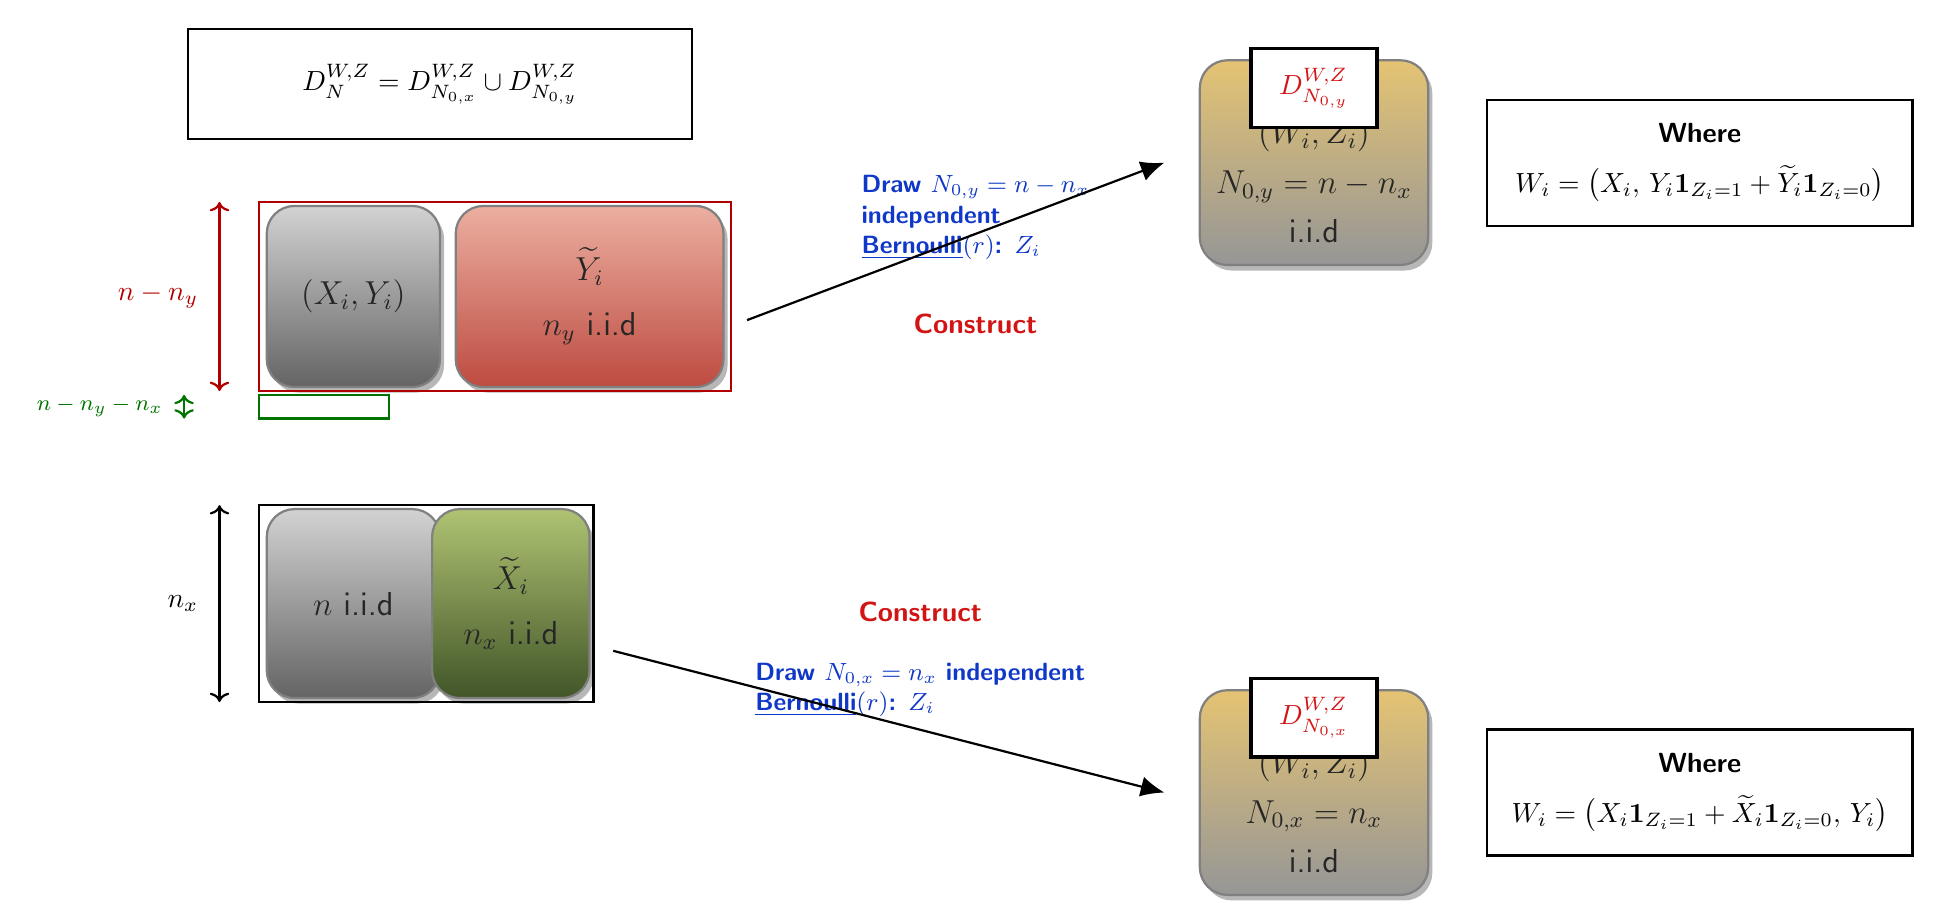
\begin{tikzpicture}[x=1cm,y=1cm]

% ---- Boite union en haut-gauche ----
\node[whitebox, minimum width=6.4cm, minimum height=1.4cm] (union) at (3.2,10.6)
  {$\mathscr{D}_N^{W,Z}=\mathscr{D}_{N_{0,x}}^{W,Z}\cup \mathscr{D}_{N_{0,y}}^{W,Z}$};

% ---- Bloc du haut : cadre rouge (X,Y)+Ytilde ----
\node[databox, top color=grayTop, bottom color=grayBot,
      minimum width=2.2cm, minimum height=2.3cm] (XY) at (2.1,7.9)
  {$(X_i,Y_i)$};
\node[databox, top color=redTop, bottom color=redBot,
      minimum width=3.4cm, minimum height=2.3cm] (Yt) at (5.1,7.9)
  {$\widetilde{Y}_i$\\[6pt] $n_y$ i.i.d};
\draw[red!70!black, thick] (0.9,6.7) rectangle (6.9,9.1);
\draw[<->, red!70!black, thick] (0.4,6.7) -- (0.4,9.1)
  node[midway, left=4pt, font=\sffamily] {$n-n_y$};

% ---- Bandeau vert intermediaire ----
\draw[green!45!black, thick] (0.9,6.35) rectangle (2.55,6.65);
\draw[<->, green!45!black, thick] (-0.05,6.35) -- (-0.05,6.65)
  node[midway, left=4pt, font=\sffamily\footnotesize] {$n-n_y-n_x$};

% ---- Bloc du bas : cadre noir n iid + Xtilde ----
\node[databox, top color=grayTop, bottom color=grayBot,
      minimum width=2.2cm, minimum height=2.4cm] (XY2) at (2.1,4.0)
  {$n$ i.i.d};
\node[databox, top color=greenTop, bottom color=greenBot,
      minimum width=2.0cm, minimum height=2.4cm] (Xt) at (4.1,4.0)
  {$\widetilde{X}_i$\\[6pt] $n_x$ i.i.d};
\draw[black, thick] (0.9,2.75) rectangle (5.15,5.25);
\draw[<->, thick] (0.4,2.75) -- (0.4,5.25)
  node[midway, left=4pt, font=\sffamily] {$n_x$};

% ---- Fleche Construct HAUT vers D_N0y ----
\node[font=\sffamily\bfseries\small, text=accentBlue, align=left] (lab1) at (10.0,8.9)
  {Draw $N_{0,y}=n-n_x$\\ independent\\ \underline{Bernoulli}$(r)$: $Z_i$};
\node[font=\sffamily\bfseries, text=accentRed] at (10.0,7.55) {Construct};
\draw[-{Latex[length=3mm,width=2.6mm]}, thick] (7.1,7.6) -- (12.4,9.6);

\node[databox, top color=goldTop, bottom color=goldBot,
      minimum width=2.9cm, minimum height=2.6cm] (D0y) at (14.3,9.6)
  {\\[8pt] $(W_i,Z_i)$\\[4pt] $N_{0,y}=n-n_x$\\[4pt] i.i.d};
\node[tagbox, minimum width=1.6cm, minimum height=1.0cm] at (14.3,10.55)
  {$\mathscr{D}_{N_{0,y}}^{W,Z}$};

\node[whitebox, minimum width=5.4cm, minimum height=1.6cm] (where1) at (19.2,9.6)
  {\textbf{Where}\\[6pt]
   $W_i=\big(X_i,\,Y_i\mathbf{1}_{Z_i=1}+\widetilde{Y}_i\mathbf{1}_{Z_i=0}\big)$};

% ---- Fleche Construct BAS vers D_N0x ----
\node[font=\sffamily\bfseries, text=accentRed] at (9.3,3.9) {Construct};
\node[font=\sffamily\bfseries\small, text=accentBlue, align=left] at (9.3,2.9)
  {Draw $N_{0,x}=n_x$ independent\\ \underline{Bernoulli}$(r)$: $Z_i$};
\draw[-{Latex[length=3mm,width=2.6mm]}, thick] (5.4,3.4) -- (12.4,1.6);

\node[databox, top color=goldTop, bottom color=goldBot,
      minimum width=2.9cm, minimum height=2.6cm] (D0x) at (14.3,1.6)
  {\\[8pt] $(W_i,Z_i)$\\[4pt] $N_{0,x}=n_x$\\[4pt] i.i.d};
\node[tagbox, minimum width=1.6cm, minimum height=1.0cm] at (14.3,2.55)
  {$\mathscr{D}_{N_{0,x}}^{W,Z}$};

\node[whitebox, minimum width=5.4cm, minimum height=1.6cm] (where2) at (19.2,1.6)
  {\textbf{Where}\\[6pt]
   $W_i=\big(X_i\mathbf{1}_{Z_i=1}+\widetilde{X}_i\mathbf{1}_{Z_i=0},\,Y_i\big)$};

\end{tikzpicture}
\caption{Construction I.I.D. (ConsIID)}
\end{figure}

\begin{figure}[htbp]
\centering
\begin{tikzpicture}[x=1cm,y=1cm]

\node[whitebox, minimum width=7.6cm, minimum height=1.4cm] (union) at (3.2,10.6)
  {$\mathscr{D}_N^{W,Z}=\mathscr{D}_{N_{0,x}}^{W,Z}\cup \mathscr{D}_{N_1}^{W,Z}\cup \mathscr{D}_{N_{0,y}}^{W,Z}$};

% ---- Bloc haut : cadre rouge (X,Y)+Ytilde ----
\node[databox, top color=grayTop, bottom color=grayBot,
      minimum width=2.2cm, minimum height=2.3cm] (XY) at (2.1,7.9)
  {$(X_i,Y_i)$};
\node[databox, top color=redTop, bottom color=redBot,
      minimum width=3.4cm, minimum height=2.3cm] (Yt) at (5.1,7.9)
  {$\widetilde{Y}_i$\\[6pt] $n_y$ i.i.d};
\draw[red!70!black, thick] (0.9,6.7) rectangle (6.9,9.1);
\draw[<->, red!70!black, thick] (0.4,6.7) -- (0.4,9.1)
  node[midway, left=4pt, font=\sffamily] {$n-n_y$};

% ---- Bandeau vert intermediaire ----
\draw[green!45!black, thick] (0.9,6.35) rectangle (2.55,6.65);
\draw[<->, green!45!black, thick] (-0.05,6.35) -- (-0.05,6.65)
  node[midway, left=4pt, font=\sffamily\footnotesize] {$n-n_y-n_x$};

% ---- Bloc bas : n iid + Xtilde ----
\node[databox, top color=grayTop, bottom color=grayBot,
      minimum width=2.2cm, minimum height=2.4cm] (XY2) at (2.1,4.0)
  {$n$ i.i.d};
\node[databox, top color=greenTop, bottom color=greenBot,
      minimum width=2.0cm, minimum height=2.4cm] (Xt) at (4.1,4.0)
  {$\widetilde{X}_i$\\[6pt] $n_x$ i.i.d};
\draw[black, thick] (0.9,2.75) rectangle (5.15,5.25);
\draw[<->, thick] (0.4,2.75) -- (0.4,5.25)
  node[midway, left=4pt, font=\sffamily] {$n_x$};

% ---- Fleche HAUT vers D_N0y ----
\node[font=\sffamily\bfseries\small, text=accentBlue, align=left] at (10.0,8.9)
  {Draw $N_{0,y}=n-n_y$\\ independent\\ \underline{Bernoulli}$(r)$: $Z_i$};
\node[font=\sffamily\bfseries, text=accentRed] at (10.0,7.55) {Construct};
\draw[-{Latex[length=3mm,width=2.6mm]}, thick] (7.1,7.6) -- (12.4,9.6);

\node[databox, top color=goldTop, bottom color=goldBot,
      minimum width=2.9cm, minimum height=2.6cm] (D0y) at (14.3,9.6)
  {\\[8pt] $(W_i,Z_i)$\\[4pt] $N_{0,y}=n-n_x$\\[4pt] i.i.d};
\node[tagbox, minimum width=1.6cm, minimum height=1.0cm] at (14.3,10.55)
  {$\mathscr{D}_{N_{0,y}}^{W,Z}$};
\node[whitebox, minimum width=5.4cm, minimum height=1.6cm] at (19.2,9.6)
  {\textbf{Where}\\[6pt]
   $W_i=\big(X_i,\,Y_i\mathbf{1}_{Z_i=1}+\widetilde{Y}_i\mathbf{1}_{Z_i=0}\big)$};

% ---- Fleche MILIEU (Construct / Framework 1) ----
\draw[-{Latex[length=3mm,width=2.6mm]}, thick] (7.1,5.5) -- (12.4,5.5);
\node[font=\sffamily\bfseries, text=accentRed] at (9.6,5.9) {Construct};
\node[font=\sffamily\bfseries\small, text=accentGreen] at (9.6,5.1)
  {Use Framework 1 (Prop. 3)};

\node[databox, top color=goldTop, bottom color=goldBot,
      minimum width=2.9cm, minimum height=2.8cm] (D1) at (14.3,5.5)
  {\\[6pt] $(W_i,Z_i)$\\[4pt]
   $N_1=\left\lfloor\dfrac{n-n_y-n_x}{2}\right\rfloor$\\[4pt] i.i.d};
\node[tagbox, minimum width=1.6cm, minimum height=1.0cm] at (14.3,6.55)
  {$\mathscr{D}_{N_1}^{W,Z}$};
\node[whitebox, minimum width=5.4cm, minimum height=1.6cm] at (19.2,5.5)
  {\textbf{Where}\\[6pt]
   $W_i=\big(X_i,\,Y_i\mathbf{1}_{Z_i=1}+Y_{i+N_1}\mathbf{1}_{Z_i=0}\big)$};

% ---- Fleche BAS vers D_N0x ----
\draw[-{Latex[length=3mm,width=2.6mm]}, thick] (5.4,3.4) -- (12.4,1.6);
\node[font=\sffamily\bfseries, text=accentRed] at (9.3,3.9) {Construct};
\node[font=\sffamily\bfseries\small, text=accentBlue, align=left] at (9.3,2.9)
  {Draw $N_{0,x}=n_x$ independent\\ \underline{Bernoulli}$(r)$: $Z_i$};

\node[databox, top color=goldTop, bottom color=goldBot,
      minimum width=2.9cm, minimum height=2.6cm] (D0x) at (14.3,1.6)
  {\\[8pt] $(W_i,Z_i)$\\[4pt] $N_{0,x}=n_x$\\[4pt] i.i.d};
\node[tagbox, minimum width=1.6cm, minimum height=1.0cm] at (14.3,2.55)
  {$\mathscr{D}_{N_{0,x}}^{W,Z}$};
\node[whitebox, minimum width=5.4cm, minimum height=1.6cm] at (19.2,1.6)
  {\textbf{Where}\\[6pt]
   $W_i=\big(X_i\mathbf{1}_{Z_i=1}+\widetilde{X}_i\mathbf{1}_{Z_i=0},\,Y_i\big)$};

\end{tikzpicture}
\caption{Construction I.I.D. augmentée à trois blocs (ConsIIDAD1)}
\end{figure}
\begin{figure}[htbp]
\centering
\begin{tikzpicture}[x=1cm,y=1cm]

\node[databox, top color=grayTop, bottom color=grayBot,
      minimum width=2.0cm, minimum height=2.4cm] (XY) at (0,0)
  {$(X_i,Y_i)$\\[6pt] $n$ i.i.d};

\draw[-{Latex[length=3mm,width=2.6mm]}, thick] (1.15,0) -- (3.1,0);
\node[font=\sffamily\bfseries, text=accentRed] at (2.1,0.45) {Construct};

\node[databox, top color=grayTop, bottom color=grayBot,
      minimum width=2.2cm, minimum height=4.4cm] (couples) at (4.6,0)
  {$(X_i,Y_j)$\\[8pt] $n^2$\\ couples};

\draw[-{Latex[length=3mm,width=2.6mm]}, thick] (5.75,1.1) -- (7.7,2.3);
\draw[-{Latex[length=3mm,width=2.6mm]}, thick] (5.75,-1.1) -- (7.7,-2.3);
\node[font=\sffamily\bfseries, text=accentRed] at (6.5,1.55) {Split};

\node[databox, top color=tealTop, bottom color=goldTop,
      minimum width=2.6cm, minimum height=2.6cm] (couplesij) at (9.4,2.6)
  {$(\widetilde{X}_i,\widetilde{Y}_j)$\\[4pt] $i\neq j$\\[4pt] $n(n-1)$\\ couples};

\node[databox, top color=grayTop, bottom color=grayBot,
      minimum width=2.2cm, minimum height=2.2cm] (couplesii) at (9.4,-2.6)
  {$(X_i,Y_i)$\\[4pt] $n$ i.i.d};

\draw[-{Latex[length=3mm,width=2.6mm]}, thick] (10.75,2.4) -- (13.3,0.35);
\node[font=\sffamily\bfseries\small, text=accentGreen, align=left] at (12.1,1.9)
  {Sample $n_0$ without\\ replacement};

\draw[-{Latex[length=3mm,width=2.6mm]}, thick] (10.75,-2.4) -- (13.3,-0.35);
\node[font=\sffamily\bfseries\small, text=accentGreen, align=left] at (12.1,-1.9)
  {Sample $n_1$ without\\ replacement};

\node[font=\sffamily\bfseries, text=accentBlue, align=center] at (14.9,1.3)
  {Draw $N=n_0+n_1$\\ independent\\ \underline{Bernoulli}$(r)$: $Z_i$};

\node[databox, top color=grayTop, bottom color=grayBot,
      minimum width=2.6cm, minimum height=4.0cm] (DWZ) at (15.2,0)
  {\\[8pt] $(W_i,Z_i)$\\[4pt] $N=n_0+n_1$\\[4pt] i.d\\ couples};
\node[tagbox, minimum width=1.6cm, minimum height=1.0cm] at (15.2,2.15)
  {$\mathscr{D}_N^{W,Z}$};

\node[whitebox, minimum width=5.6cm, minimum height=1.6cm] at (20.4,-1.6)
  {\textbf{Where}\\[6pt]
   $W_i=\big(X_i,\,Y_i\mathbf{1}_{Z_i=1}+\widetilde{Y}_i\mathbf{1}_{Z_i=0}\big)$};

\end{tikzpicture}
\caption{Construction par appariement de couples (ConsIIDAD3)}
\end{figure}
\begin{figure}[htbp]
\centering
\begin{tikzpicture}[x=1cm,y=1cm]

\node[whitebox, minimum width=7.6cm, minimum height=1.4cm] (union) at (3.2,10.6)
  {$\mathscr{D}_N^{W,Z}=\mathscr{D}_{N_{0,x}}^{W,Z}\cup \mathscr{D}_{N_1}^{W,Z}\cup \mathscr{D}_{N_{0,y}}^{W,Z}$};

% ---- Bloc haut : cadre rouge (X,Y)+Ytilde ----
\node[databox, top color=grayTop, bottom color=grayBot,
      minimum width=2.2cm, minimum height=2.3cm] (XY) at (2.1,7.9)
  {$(X_i,Y_i)$};
\node[databox, top color=redTop, bottom color=redBot,
      minimum width=3.4cm, minimum height=2.3cm] (Yt) at (5.1,7.9)
  {$\widetilde{Y}_i$\\[6pt] $n_y$ i.i.d};
\draw[red!70!black, thick] (0.9,6.7) rectangle (6.9,9.1);
\draw[<->, red!70!black, thick] (0.4,6.7) -- (0.4,9.1)
  node[midway, left=4pt, font=\sffamily] {$n-n_y$};

% ---- Bandeau vert intermediaire ----
\draw[green!45!black, thick] (0.9,6.35) rectangle (2.55,6.65);
\draw[<->, green!45!black, thick] (-0.05,6.35) -- (-0.05,6.65)
  node[midway, left=4pt, font=\sffamily\footnotesize] {$n-n_y-n_x$};

% ---- Bloc bas : n iid + Xtilde ----
\node[databox, top color=grayTop, bottom color=grayBot,
      minimum width=2.2cm, minimum height=2.4cm] (XY2) at (2.1,4.0)
  {$n$ i.i.d};
\node[databox, top color=greenTop, bottom color=greenBot,
      minimum width=2.0cm, minimum height=2.4cm] (Xt) at (4.1,4.0)
  {$\widetilde{X}_i$\\[6pt] $n_x$ i.i.d};
\draw[black, thick] (0.9,2.75) rectangle (5.15,5.25);
\draw[<->, thick] (0.4,2.75) -- (0.4,5.25)
  node[midway, left=4pt, font=\sffamily] {$n_x$};

% ---- Fleche HAUT vers D_N0y ----
\node[font=\sffamily\bfseries\small, text=accentBlue, align=left] at (10.0,8.9)
  {Draw $N_{0,y}=n-n_y$\\ independent\\ \underline{Bernoulli}$(r)$: $Z_i$};
\node[font=\sffamily\bfseries, text=accentRed] at (10.0,7.55) {Construct};
\draw[-{Latex[length=3mm,width=2.6mm]}, thick] (7.1,7.6) -- (12.4,9.6);

\node[databox, top color=goldTop, bottom color=goldBot,
      minimum width=2.9cm, minimum height=2.6cm] (D0y) at (14.3,9.6)
  {\\[8pt] $(W_i,Z_i)$\\[4pt] $N_{0,y}=n-n_x$\\[4pt] i.i.d};
\node[tagbox, minimum width=1.6cm, minimum height=1.0cm] at (14.3,10.55)
  {$\mathscr{D}_{N_{0,y}}^{W,Z}$};
\node[whitebox, minimum width=5.4cm, minimum height=1.6cm] at (19.2,9.6)
  {\textbf{Where}\\[6pt]
   $W_i=\big(X_i,\,Y_i\mathbf{1}_{Z_i=1}+\widetilde{Y}_i\mathbf{1}_{Z_i=0}\big)$};

% ---- Fleche MILIEU (Construct / Framework 1) ----
\draw[-{Latex[length=3mm,width=2.6mm]}, thick] (7.1,5.5) -- (12.4,5.5);
\node[font=\sffamily\bfseries, text=accentRed] at (9.6,5.9) {Construct};
\node[font=\sffamily\bfseries\small, text=accentGreen] at (9.6,5.1)
  {Use Framework 1 (Prop. 3)};

\node[databox, top color=goldTop, bottom color=goldBot,
      minimum width=2.9cm, minimum height=2.8cm] (D1) at (14.3,5.5)
  {\\[6pt] $(W_i,Z_i)$\\[4pt]
   $N_1=\left\lfloor\dfrac{n-n_y-n_x}{2}\right\rfloor$\\[4pt] i.i.d};
\node[tagbox, minimum width=1.6cm, minimum height=1.0cm] at (14.3,6.55)
  {$\mathscr{D}_{N_1}^{W,Z}$};
\node[whitebox, minimum width=5.4cm, minimum height=1.6cm] at (19.2,5.5)
  {\textbf{Where}\\[6pt]
   $W_i=\big(X_i,\,Y_i\mathbf{1}_{Z_i=1}+Y_{i+N_1}\mathbf{1}_{Z_i=0}\big)$};

% ---- Fleche BAS vers D_N0x ----
\draw[-{Latex[length=3mm,width=2.6mm]}, thick] (5.4,3.4) -- (12.4,1.6);
\node[font=\sffamily\bfseries, text=accentRed] at (9.3,3.9) {Construct};
\node[font=\sffamily\bfseries\small, text=accentBlue, align=left] at (9.3,2.9)
  {Draw $N_{0,x}=n_x$ independent\\ \underline{Bernoulli}$(r)$: $Z_i$};

\node[databox, top color=goldTop, bottom color=goldBot,
      minimum width=2.9cm, minimum height=2.6cm] (D0x) at (14.3,1.6)
  {\\[8pt] $(W_i,Z_i)$\\[4pt] $N_{0,x}=n_x$\\[4pt] i.i.d};
\node[tagbox, minimum width=1.6cm, minimum height=1.0cm] at (14.3,2.55)
  {$\mathscr{D}_{N_{0,x}}^{W,Z}$};
\node[whitebox, minimum width=5.4cm, minimum height=1.6cm] at (19.2,1.6)
  {\textbf{Where}\\[6pt]
   $W_i=\big(X_i\mathbf{1}_{Z_i=1}+\widetilde{X}_i\mathbf{1}_{Z_i=0},\,Y_i\big)$};

\end{tikzpicture}
\caption{Construction I.I.D. augmentée à trois blocs (ConsIIDAD1)}
\end{figure}


\end{document}